\documentclass{beamer}

% Thème
\usetheme{metropolis} % Un thème moderne
\usecolortheme{dove} % Couleurs épurées

% Paquets supplémentaires
\usepackage{graphicx}
\usepackage{booktabs}
\usepackage[french]{babel}

% Required package
\usepackage[absolute,overlay]{textpos}

\usepackage{fontspec}
%\setmainfont{helvetica}

% Informations sur la présentation
\title{1924B Mini Boîte Noire}
\subtitle{Enregistreur de données de vol}
\author{Ali Zoubir}
\institute{\textbf{ETML-\textcolor{red}{ES}}}
\date{\today}

\begin{document}
	
\begin{frame}[plain]
	\maketitle
	\begin{textblock*}{2cm}(9cm,5cm) % {block width} (coords)	
		\includegraphics[width=1\linewidth]{../figures/AMPA}
	\end{textblock*}
	\begin{textblock*}{2cm}(9cm,6.5cm) % {block width} (coords)	
		
\includegraphics[width=1\linewidth]{../figures/ETML-ES}
	\end{textblock*}
\end{frame}

\begin{frame}{Sommaire}
	\tableofcontents
\end{frame}

\section{Introduction}

\begin{frame}{Introduction}	
	\begin{textblock*}{4cm}(1cm,1cm) % {block width} (coords)	
	\begin{figure}[h]
		\centering
		\includegraphics[width=1\linewidth]{../figures/boite-noire}
		\caption{Boîte noire}
		\label{fig:boite-noire}
	\end{figure}
	\end{textblock*}
	
	\begin{textblock*}{7cm}(5.5cm,1.5cm) % {block width} (coords)
		Les enregistreurs de données de vol jouent un rôle crucial dans la sécurité aérienne et la compréhension des phénomènes aéronautiques en capturant de manière inaltérable des informations vitales. 
		
		Ce projet a pour but la collecte et le stockage des données de mesures et de \textcolor{blue}{localisation} d'un aéronef au moyen d'une centrale \textcolor{blue}{inertielle} et d'un système de positionnement GPS/GNSS.		
	\end{textblock*}
\end{frame}

\begin{frame}{Principe}	
	\begin{textblock*}{4.5cm}(1cm,1cm) % {block width} (coords)
	\begin{figure}[h]
		\centering
		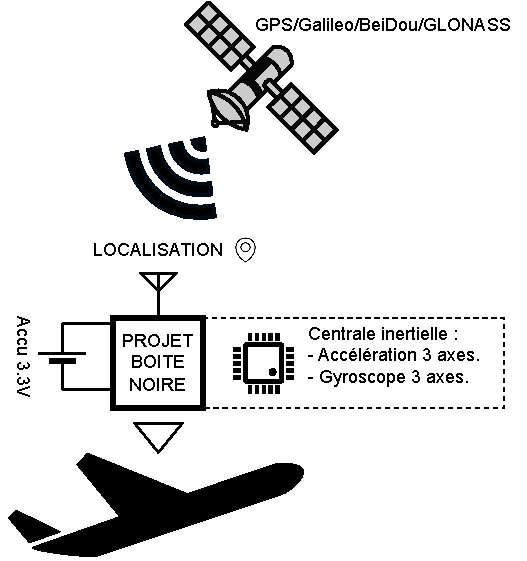
\includegraphics[width=1\linewidth]{../figures/cdc/schema_principe}
		\caption{Schéma de principe.}
		\label{fig:schemaprincipe}
	\end{figure}
	\end{textblock*}

	\begin{textblock*}{7cm}(5.5cm,1.5cm) 
	\begin{itemize}
		\item Données de localisation, trajectoire.
		\item Accéléromètre et Gyroscope.
		\item Miniaturisation.
		\item Bonne autonomie / Low power.
		\item Configuration des temps de sauvegardes.
		\item Charge, lecture et configuration par USB-C.
	\end{itemize}
	\end{textblock*}
\end{frame}

\section{Pré-étude}
\begin{frame}{Schéma bloc}
	\begin{figure}[h]
		\centering
		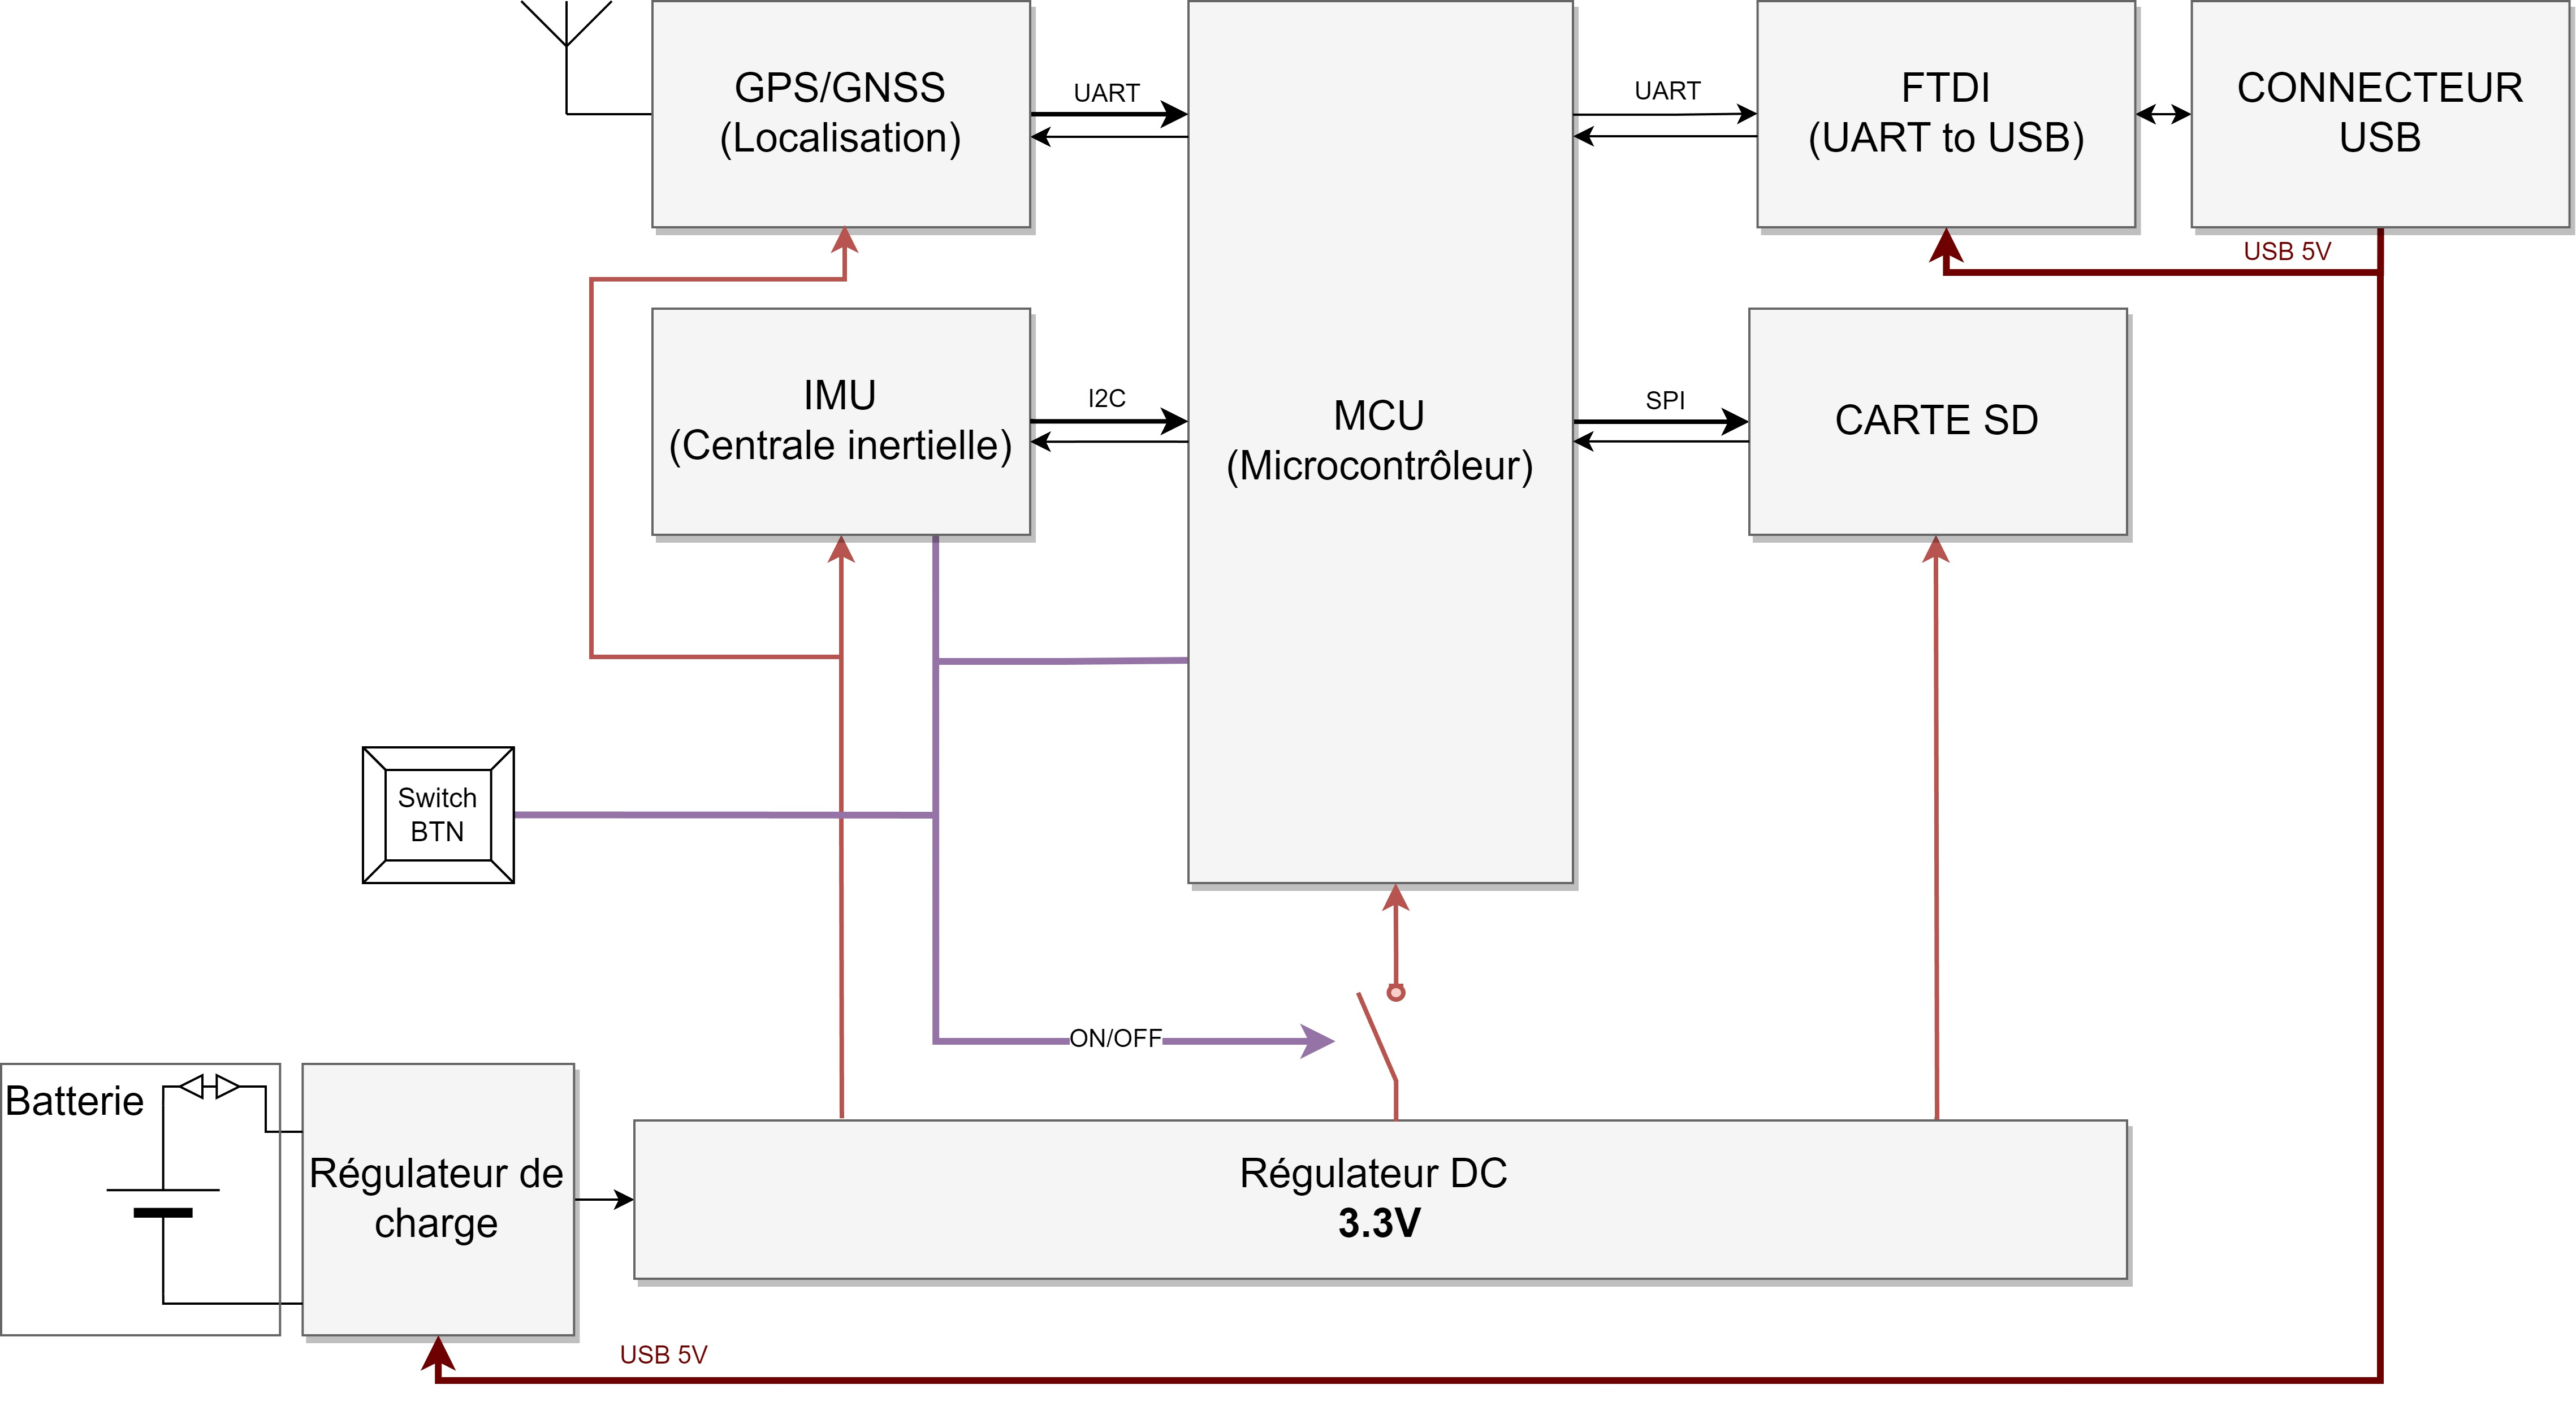
\includegraphics[width=1\textwidth]{../figures/cdc/blocs_grossiers_no_antenna}
		\caption{Schéma bloc.}
		\label{fig:schbloc}
	\end{figure}
\end{frame}

\begin{frame}{Choix des composants clés}
	\begin{tabular}{lll}
		Microcontrôleur &:& PIC32MX274F256D \\
		Centrale inertielle &:& BNO055 \\
		GNSS &:& CAM-M8C-0 \\
		Carte SD &:& 256MB \\
		Batterie &:& LI-ION 1600mAh \\
		Régulateur &:& MCP73871T-2CCI/ML\\
	\end{tabular}
\end{frame}

\begin{frame}{Microcontrôleur}
	\begin{figure}[h]
		\centering
		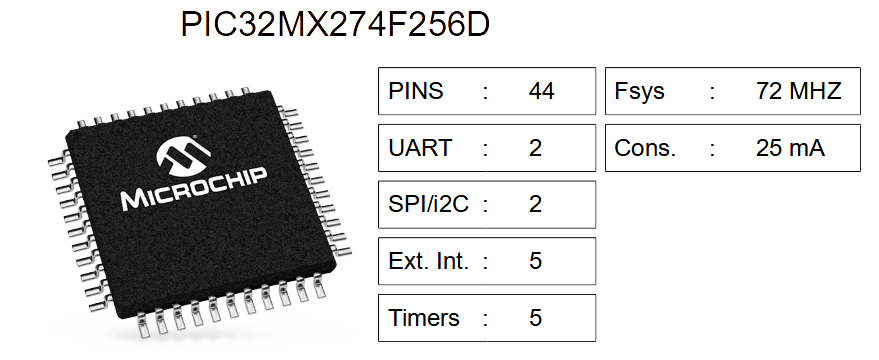
\includegraphics[width=0.7\linewidth]{../figures/pre_etude/Carac_PIC32}
		\caption{Caractéristiques PIC32.}
	\end{figure}
	Le MCU choisis dispose de différentes configurations de gestion de puissance, notamment des modes d'économie d'énergie, afin de permettre une meilleure autonomie. 
\end{frame}

\begin{frame}{Centrale inertielle}
	\begin{center}
		\begin{figure}[h]
			\centering
			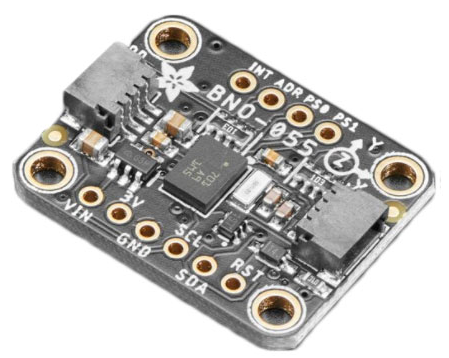
\includegraphics[width=0.25\linewidth]{../figures/pre_etude/BNO055_Adafruit}
			\caption{Illustration BNO055.}
		\end{figure} \vspace*{-2mm}
		
		\underline{Caractéristiques importantes :} \\
		\resizebox{.5\textwidth}{!}{\begin{tabular}{l l l l}
			Résolution gyroscope & : & 16 & [bits] \\
			Résolution accéléromètre & : & 14 & [bits] \\
			Résolution magnétomètre & : & $\sim$0.3 & [$\mu$T] \\
			$I_{DD}$ & : & 12.3 & [mA] \\
			Dérive de température & : & $\pm$ 0.03 & [\%/K] \\ 
			Dérive accéléromètre & : & 0.2 & [\%/V] \\
			Dérive gyroscope & : & <0.4 & [\%/V]
		\end{tabular}} \\
	\end{center}
\end{frame}

\begin{frame}{GNSS}
	\begin{figure}[h]
		\centering
		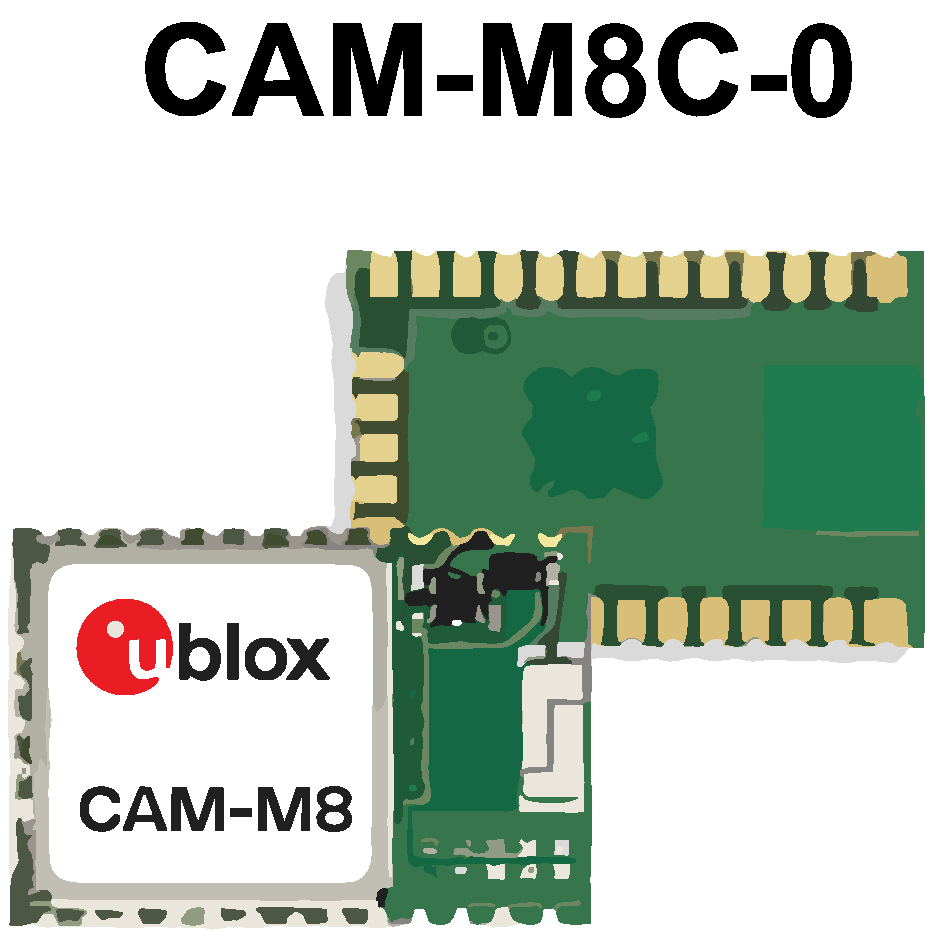
\includegraphics[width=0.25\linewidth]{../figures/pre_etude/img_gnss_crp}
	\end{figure}
	
	\begin{figure}[h]
		\centering
		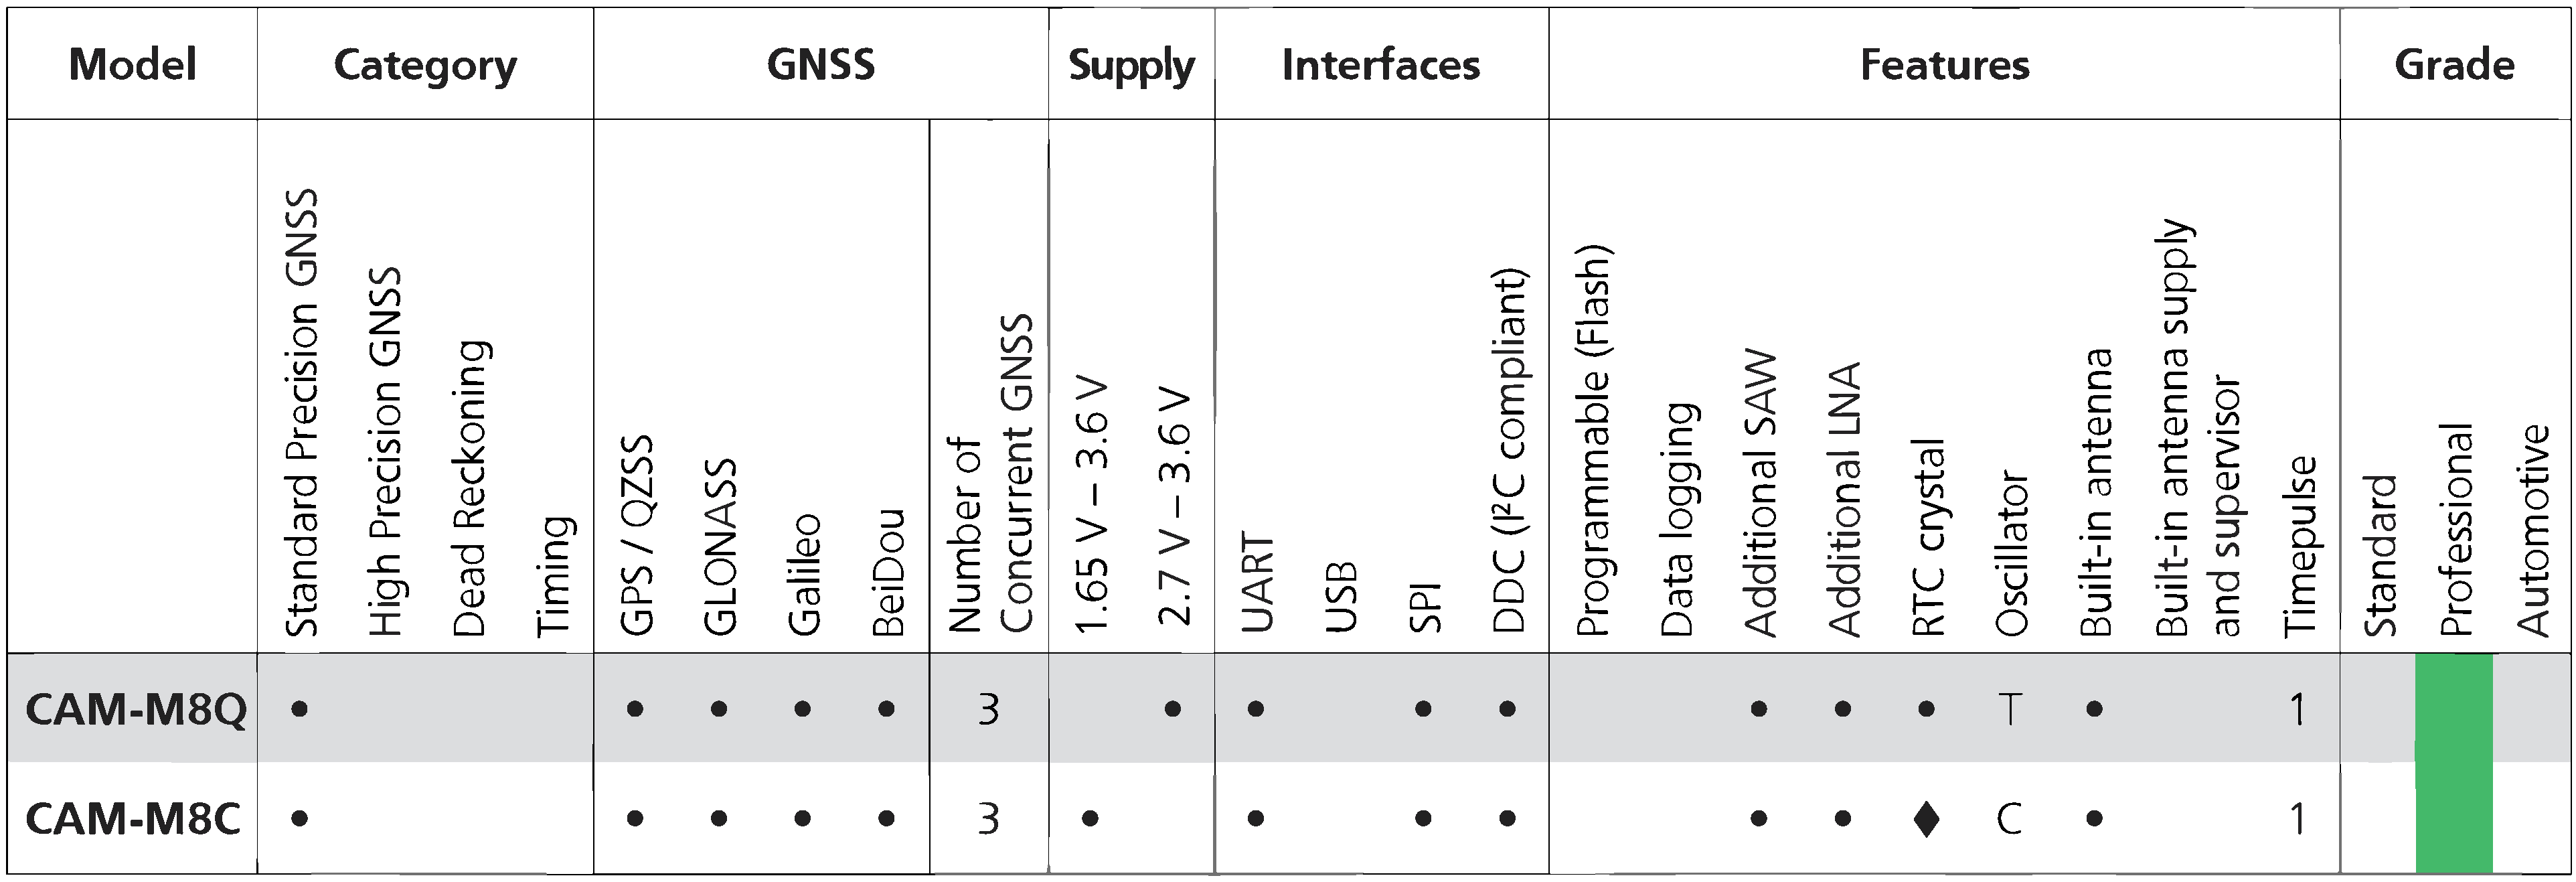
\includegraphics[width=.9\linewidth]{../figures/pre_etude/carac_GNSS}
		\caption{Caractéristiques du GNSS.}
		\label{fig:caracgnss}
	\end{figure}
\end{frame}

\begin{frame}{Carte SD}
	\begin{center}
	\resizebox{.4\textwidth}{!}{\begin{tabular}{lrl}
		$S_{SD}$ & $256$ & $[MB]$ \\
		$S_{gyro}$ & $16$ & $[Bytes]$ \\
		$S_{accel}$ & $16$ & $[Bytes]$ \\
		$S_{gnss}$ & $\sim100$ & $[Bytes]$ \\
		$T_{inertiel}$ & $0.5$ & $[s]$ \\
		$T_{gnss}$ & $5$ & $[s]$ \\
		$T_{mesMin}$ & $900$ & $[s]$ \\
	\end{tabular}}
	\end{center}\vspace*{-3mm}
	
	\begin{equation*}
		S_{single} = \frac{T_{gnss}}{T_{inertiel}}S_{accel} + S_{gnss} = \frac{5}{0.5}16 + 100 = 260 \; [Bytes]
	\end{equation*}\vspace*{-10mm}
	
	\begin{equation*}
		S_{mesures} = \frac{S_{single}}{T_{gnss}} * T_{mesMin} = \frac{260}{5} * 900 = 46'800 \; [Bytes] = 49.8 \; [KB]
	\end{equation*}\vspace*{-10mm}
	
	\begin{equation*}
		T_{mesures} = \frac{S_{SD}*T_{gnss}}{S_{single}} = \frac{256*10^6*5}{260} = \sim82'051 \; Minutes = \sim1368 \; H.
	\end{equation*}
\end{frame}

\begin{frame}{Batterie}
	\begin{center}
		\underline{Liste des consommations principales} \\
		\begin{table}[h]
			\centering
			\begin{tabular}{lrll}
				Microcontrôleur & 24 & [mA] & Typ. \\
				Carte-SD & ~100 & [mA] & Max. \\
				Carte-SD & ~60 & [mA] & Moyenne \\
				IMU & 12.3 & [mA] & Typ. \\
				GNSs & 71 & [mA] & Max. \\
				GNSS & 29 & [mA] & Typ. \\
				\hline
				Totale max & \underline{207.3} & [mA] & Max. \\
				Totale moyennes & \underline{125.3} & [mA] & Moyenne \\
				\hline
			\end{tabular}
			\caption{Tableau des consommations de courant.}
			\label{tab:consommateur}
		\end{table}
	\end{center}
	Temps minimum avec tolérance désiré : $10h \Rightarrow$ $\min\sim1300mAh$
\end{frame}

\section{Conclusion}
\begin{frame}{Conclusion}
	Résumons ce que nous avons appris.
\end{frame}

\begin{frame}[standout]
	Questions?
\end{frame}
	
\end{document}
